\begin{figure}[tbp]
\centering
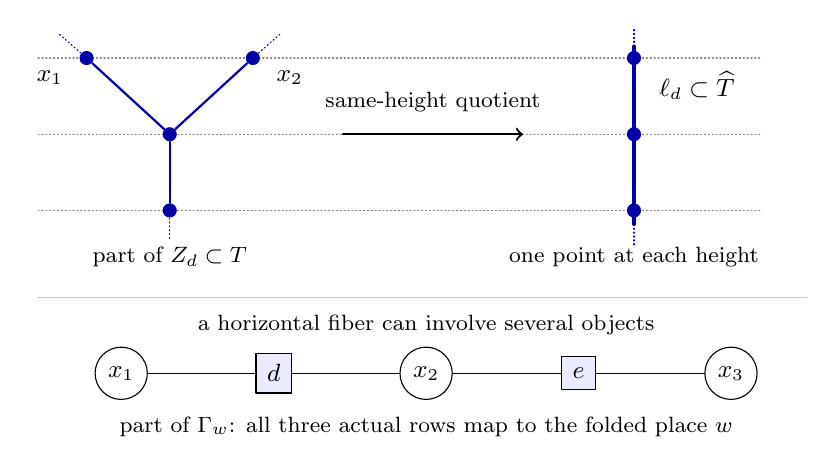
\begin{tikzpicture}[x=.88cm,y=.88cm,font=\small,
  every node/.style={align=center},line cap=round,line join=round,
  row/.style={draw,circle,fill=white,inner sep=3pt},
  object/.style={draw,rectangle,fill=blue!8,inner sep=4pt},
  dot/.style={circle,fill=blue!65!black,inner sep=1.8pt}]
  \draw[densely dotted,gray] (.4,-.15)--(10.85,-.15);
  \draw[densely dotted,gray] (.4,-1.25)--(10.85,-1.25);
  \draw[densely dotted,gray] (.4,-2.35)--(10.85,-2.35);
  \node[dot] (za) at (1.1,-.15) {};
  \node[dot] (zb) at (3.5,-.15) {};
  \node[dot] (zc) at (2.3,-1.25) {};
  \node[dot] (zd) at (2.3,-2.35) {};
  \draw[thick,blue!65!black] (za)--(zc)--(zb);
  \draw[thick,blue!65!black] (zc)--(zd);
  \draw[densely dotted,blue!65!black] (za)--(.7,.2);
  \draw[densely dotted,blue!65!black] (zb)--(3.9,.2);
  \draw[densely dotted,blue!65!black] (zd)--(2.3,-2.78);
  \node[anchor=east] at (.9,-.43) {$x_1$};
  \node[anchor=west] at (3.7,-.43) {$x_2$};
  \node[font=\footnotesize] at (2.3,-3.02) {part of $Z_d\subset T$};
  \draw[->,thick] (4.8,-1.25)--(7.4,-1.25);
  \node[fill=white,inner sep=2pt,font=\footnotesize] at (6.1,-.78)
    {same-height quotient};
  \draw[very thick,blue!65!black] (9,-2.55)--(9,.02);
  \draw[densely dotted,blue!65!black] (9,-2.55)--(9,-2.85);
  \draw[densely dotted,blue!65!black] (9,.02)--(9,.28);
  \node[dot] at (9,-.15) {};
  \node[dot] at (9,-1.25) {};
  \node[dot] at (9,-2.35) {};
  \node[anchor=west,fill=white,inner sep=2pt] at (9.28,-.55)
    {$\ell_d\subset\widehat T$};
  \node[font=\footnotesize] at (9,-3.02) {one point at each height};

  \draw[gray!45] (.4,-3.6)--(11.5,-3.6);
  \node[font=\footnotesize] at (6,-4.0)
    {a horizontal fiber can involve several objects};
  \node[row] (x1) at (1.6,-4.7) {$x_1$};
  \node[object] (d) at (3.8,-4.7) {$d$};
  \node[row] (x2) at (6,-4.7) {$x_2$};
  \node[object] (e) at (8.2,-4.7) {$e$};
  \node[row] (x3) at (10.4,-4.7) {$x_3$};
  \draw (x1)--(d)--(x2)--(e)--(x3);
  \node[font=\footnotesize] at (6,-5.47)
    {part of $\Gamma_w$: all three actual rows map to the folded place $w$};
\end{tikzpicture}
\caption{Strict folding is the transitive quotient generated by identifying
same-height points within each $Z_d$. The upper panel shows the image
of one subtree; horizontal guides indicate height. It does not identify
arbitrary equal-height points of $T$. The lower panel records how two
objects can make three actual rows equivalent at one height: an incidence
$x,d$ means $x\in Z_d$. Such incidence chains describe the horizontal
fiber $\Gamma_w$, whose stabilizer and homology are analyzed below.}
\label{fig:row-refinement-folding}
\end{figure}
